\documentclass[a4paper,11pt]{article}

% ------------------------------
% Geometry and Page Layout
% ------------------------------
\usepackage{geometry}
\geometry{left=1in, right=1in, top=1in, bottom=1in} % Set 1-inch margins
\usepackage{fancyhdr}   % Header and footer customization
\usepackage{pdflscape}  % Landscape pages
\usepackage{everypage}  % Add hooks to every page

% ------------------------------
% Font and Typography
% ------------------------------
\usepackage{mathptmx}   % Use Times New Roman font (or Computer Modern by default)
\renewcommand{\baselinestretch}{1.5} % Line spacing
\usepackage[utf8]{inputenc} % UTF-8 support
\usepackage{tocloft}
\usepackage[normalem]{ulem}

% ------------------------------
% For customizing titles
% ------------------------------
\usepackage{titlesec}
% Redefine \section to be unnumbered but still included in TOC

% ------------------------------
% Date Handling
% ------------------------------
\usepackage[english]{datetime2}
\DTMnewdatestyle{mydateA}{%
  \renewcommand*{\DTMdisplaydate}[4]{%
    \DTMtwodigits{##3}/\DTMtwodigits{##2}/##1}%
  \renewcommand*{\DTMDisplaydate}{\DTMdisplaydate}%
}
\DTMnewdatestyle{mydateB}{%
  \renewcommand*{\DTMdisplaydate}[4]{%
    \DTMtwodigits{##3} \DTMenglishmonthname{##2} ##1}%
  \renewcommand*{\DTMDisplaydate}{\DTMdisplaydate}%
}

% ------------------------------
% Color and Graphics
% ------------------------------
\usepackage[table]{xcolor}
\definecolor{mygreen}{rgb}{0.82, 0.94, 0.75}
\definecolor{mygreen2}{rgb}{0.67, 0.88, 0.69}
\definecolor{codegreen}{rgb}{0,0.94,0}
\definecolor{codegray}{rgb}{0.5,0.5,0.5}
\definecolor{codepurple}{rgb}{0.58,0,0.82}
\definecolor{backcolour}{rgb}{0.95,0.95,0.92}
\usepackage{graphicx}   % For including figures
\graphicspath{{}}       % Set graphic paths
\DeclareGraphicsExtensions{.pdf,.jpeg,.png,.jpg}
\usepackage{tikz}       % For custom drawings and diagrams
\usepackage{subcaption}  % For subfigures
\usepackage{float}

% ------------------------------
% Mathematics
% ------------------------------
\usepackage{amsmath}    % Mathematical symbols and environments
\usepackage{amssymb}    % Additional math symbols
\usepackage{yhmath}     % Extended math fonts
\usepackage{extarrows}  % Extensible arrows
\usepackage{esint}      % Integrals
\usepackage{bigints}    % Large integral symbols
\usepackage{mathrsfs}   % Script math font

% ------------------------------
% Code Formatting
% ------------------------------
\usepackage{listings}   % Code listings
\lstdefinestyle{mystyle}{
    backgroundcolor=\color{backcolour},   
    commentstyle=\color{green!50!black},
    keywordstyle=\color{blue},
    numberstyle=\tiny\color{codegray},
    stringstyle=\color{red},
    basicstyle=\ttfamily\footnotesize, % Adjusting the code size here
    breakatwhitespace=false,         
    breaklines=true,                 
    captionpos=b,                    
    keepspaces=true,                 
    numbers=left,                    
    numbersep=5pt,                  
    showspaces=false,                
    showstringspaces=false,
    showtabs=false,                  
    tabsize=2,
    frame=single,
    captionpos=b
}
\lstset{style=mystyle}

% ------------------------------
% Bibliography Management
% ------------------------------
\usepackage[backend=biber, 
            isbn=false, 
            url=true, 
            doi=true, 
            giveninits=true, 
            sorting=none]{biblatex}
\addbibresource{ref.bib}

% Optional: Customize title formatting to keep hyperlinks intact
\newbibmacro{string+doi}[1]{%
  \iffieldundef{doi}{#1}
  {\href{https://doi.org/\thefield{doi}}{#1}}}

\DeclareFieldFormat{title}{\usebibmacro{string+doi}{\mkbibemph{#1}}}
\DeclareFieldFormat[article]{title}{\usebibmacro{string+doi}{\mkbibquote{#1}}}
\DeclareFieldFormat[article,periodical]{volume}{\mkbibbold{#1}}
\DeclareFieldFormat[article,periodical]{number}{\mkbibbold{#1}}

% ------------------------------
% Packages for Tables
% ------------------------------
\usepackage{array}      % Extended column definitions
\usepackage{tabularx}   % Table with adjustable-width columns
\usepackage{longtable}  % Tables spanning multiple pages
\usepackage{booktabs}   % Formal tables
\usepackage{arydshln}   % Dashed lines in tables
\usepackage{multirow}   % Multi-row cells
\usepackage{makecell}   % Enhanced table cells
\usepackage{tasks}      % Task lists within tables

% ------------------------------
% Custom Commands and Settings
% ------------------------------
\newcommand{\checkbox}{\makebox[0.5cm]{\strut $\square$}} % Custom checkbox command
\newcommand{\RotatePagenumber}{%
  \ifdim\textwidth=\linewidth
    % Do nothing if text width equals line width
  \else
    \begingroup
    \dimendef\margins=0
    \ifodd\value{page}
      \margins=\oddsidemargin
    \else
      \margins=\evensidemargin
    \fi
    \raisebox{\dimexpr -\topmargin-\headheight-\headsep-\footskip-1cm}[0pt][0pt]{%
      \rlap{\hspace{\dimexpr \margins + \textheight + \footskip + \marginparwidth}%
      \llap{\rotatebox{90}{\thepage}}}}%
    \endgroup
  \fi
}
\AddEverypageHook{\RotatePagenumber} % Apply custom page numbering

% ------------------------------
% Color and Hyperlink Settings
% ------------------------------
\usepackage[colorlinks]{hyperref}
\hypersetup{
    linkcolor=blue,   % Color for internal links
    citecolor=red,    % Color for citations
    urlcolor=purple,  % Color for URLs
}

% ------------------------------
% cross reference
% ------------------------------
\usepackage[nameinlink,capitalize]{cleveref} %cross reference showing Eq. (1) etc.

% ------------------------------
% Start Document
% ------------------------------
\begin{document}
\thispagestyle{empty}
\DTMsetdatestyle{mydateA}

%%%%%%%%%%%%%%%%%%%%%%%%%%%%%%%%%%%%%%%%%%%%%%%%%%%%%%%%%%%%%%%%%%%%%%%%%%%%%%%%%%%%%%%%
% Slip
%%%%%%%%%%%%%%%%%%%%%%%%%%%%%%%%%%%%%%%%%%%%%%%%%%%%%%%%%%%%%%%%%%%%%%%%%%%%%%%%%%%%%%%%
%SCHOOL OF PHYSICS -- LEVEL 200 PHYSICS LABORATORY REPORT SLIP
\begin{center}
    \textbf{SCHOOL OF PHYSICS -- LEVEL 200 PHYSICS LABORATORY REPORT SLIP} \\
    \textbf{FOR ZCT 293/2 AND ZCT 294/2}
\end{center}

\begin{table}[h]
\begin{center}
\resizebox{\textwidth}{!}{
\begin{tabular}{|llllllllllllllllllll|}
\hline
\multicolumn{20}{|l|}{\textbf{Instructions to student:} Please make sure you fill in the form completely.} \\
\multicolumn{20}{|l|}{\textbf{Instructions to lecturer:} Kindly record the numerical marks in the rubric assessment form, not here.} \\ \hline
\multicolumn{20}{|c|}{
  \centering{\textbf{PARTICULARS}}
}                                                                                                                                      \\ \hline
Name & :\,\,TAN WEI LIANG & \multicolumn{18}{l|}{}                                                                                                                                                                        
\\ \hline
Matric no. & :\,\,22302889  & \multicolumn{18}{l|}{}                                                                                                                                                                        
\\ \hline
Group& :\,\,W2  & \multicolumn{18}{l|}{}                                                                                                                                                                        
\\ \hline
Expt. Code & :\,\,2OS2 & \multicolumn{18}{l|}{}                                                                                                                                                                        
\\ \hline
Expt. Title & :\,\,DIFFRACTION GRATING SPECTROMETER & \multicolumn{18}{l|}{}                                                                                                                                                                        
\\ \hline
Lecturer in charge & :\,\,DR. SITI AZRAH MOHAMAD SAMSURI  & \multicolumn{18}{l|}{}                                                                                                                                                                        
\\ \hline
Report due date & :\,\,\today & \multicolumn{18}{l|}{}                                                                                                                                                                        
\\ \hline
\multicolumn{11}{|c|}{\textbf{Experiment (\checkmark)}} & \multicolumn{9}{c|}{\textbf{Lab Report Grade (\checkmark)}} \\ 
\hline
\multicolumn{11}{|c|}{1 $\square$ \quad 2 $\square$ \quad 3 $\text{\rlap{$\checkmark$}}\square$  \quad 4 $\square$ \quad 5 $\square$ \quad 6 $\square$} & 

\multicolumn{1}{l|}{A} & \multicolumn{1}{l|}{$\square$} &
\multicolumn{1}{l|}{A$-$} & \multicolumn{1}{l|}{$\square$} &
\multicolumn{1}{l|}{B$+$} & \multicolumn{1}{l|}{$\square$} &
\multicolumn{1}{l|}{B} & \multicolumn{1}{l|}{$\square$} 
&\multicolumn{1}{l|}{}
\\ \hline
\multicolumn{11}{|l|}{} & 

\multicolumn{1}{l|}{B$-$} & \multicolumn{1}{l|}{$\square$} &
\multicolumn{1}{l|}{C$+$} & \multicolumn{1}{l|}{$\square$} &
\multicolumn{1}{l|}{C} & \multicolumn{1}{l|}{$\square$} &
\multicolumn{1}{l|}{C$-$} & \multicolumn{1}{l|}{$\square$} 
&\multicolumn{1}{l|}{}
\\ \hline

\multicolumn{11}{|c|}{} & 

\multicolumn{1}{l|}{D$+$} & \multicolumn{1}{l|}{$\square$} &
\multicolumn{1}{l|}{D} & \multicolumn{1}{l|}{$\square$} &
\multicolumn{1}{l|}{D$-$} & \multicolumn{1}{l|}{$\square$} &
\multicolumn{1}{l|}{F} & \multicolumn{1}{l|}{$\square$} 
&\multicolumn{1}{l|}{}
\\ \hline
\multicolumn{20}{|c|}{} \\\hline 
\multicolumn{10}{|c|}{Date Received (Stamp):} & 
\multicolumn{10}{c|}{Comments:}  \\ \hline   
\multicolumn{10}{|c|}{} & 
\multicolumn{10}{c|}{}\\
\multicolumn{10}{|c|}{} & 
\multicolumn{10}{c|}{}\\
\multicolumn{10}{|c|}{} & 
\multicolumn{10}{c|}{}\\
\multicolumn{10}{|c|}{} & 
\multicolumn{10}{c|}{}\\
\multicolumn{10}{|c|}{} & 
\multicolumn{10}{c|}{}\\
\multicolumn{10}{|c|}{} & 
\multicolumn{10}{c|}{}\\\hline     
\end{tabular}
}
\end{center}
\end{table}

\newpage

\thispagestyle{empty}

\begin{center}
\textbf {\Large REPORT SUBMISSION FORM}
\end{center}

\begin{figure}[ht]
\begin{flushright}

\includegraphics[width=0.28\textwidth]{USMlogo}
\end{flushright}
\end{figure}

\large
\begin{tabular}{lcl}
Name & : &\dotuline{TAN WEi LIANG\hfill}\\
\\
Partner's Name &: &\dotuline{TAN SHUENN PYNG\hfill}\\
\\
Group& : &\dotuline{W2\hfill}\\
\\
Experiment Code& :&\dotuline{2OS6\hfill}\\
\\
Experiment Title&: &\dotuline{DIFFRACTION GRATING SPECTROMETER\hfill}\\
\\
Lecturer's/Examiner's&: &\dotuline{DR. SITI AZRAH MOHAMAD SAMSURI\hfill}\\ 
Name\\
\\
Starting Date &: &\dotuline{20/11/2024\hfill}\\
(1st session)\\
\\
Ending Date &: &\dotuline{27/11/2024\hfill}\\
(2nd session)\\
\\
Submission Date &: &\dotuline{$\today$\hfill}\\
\\
\end{tabular}


\newpage
\thispagestyle{empty}

\begin{center}
\textbf{\Large DECLARATION OF ORIGINALITY}
\end{center}
\bigskip
I, \textbf{TAN WEI LIANG 22302889}
hereby declare that this laboratory report is my own work. I further declare that:

\begin{enumerate}
    \item The references/bibliography reflect the sources I have consulted, and
    \item I also certify that this report has not previously been submitted for assessment in this or any other units, and that I have not copied in part or whole or otherwise plagiarized the work of other students and/or persons.
    \item Sections with no source referrals are my own ideas, arguments, and/or conclusions.
\end{enumerate}

\bigskip
\begin{figure}[htbp]
\hspace{35mm}
\includegraphics[width=0.1\linewidth]{signature}
\label{6}
\vspace{-12mm}
\end{figure}
\noindent Signature: \hrulefill \hfill Date: \uline{$\today$}

\newpage

%%%%%%%%%%%%%%%%%%%%%%%%%%%%%%%%%%%%%%%%%%%%%%%%%%%%%%%%%%%%%%%%%%%%%%%%%%%%%%%%%%%%%%%%%%%
%Reporty Content
%%%%%%%%%%%%%%%%%%%%%%%%%%%%%%%%%%%%%%%%%%%%%%%%%%%%%%%%%%%%%%%%%%%%%%%%%%%%%%%%%%%%%%%%%%%
\thispagestyle{empty}

\DTMsetdatestyle{mydateB}

%%%
\begin{center}
\vspace*{1cm}
\textbf{\Large DIFFRACTION GRATING SPECTROMETER}

\vspace{3.0cm}
\textbf{\Large By}\\

\vspace{3.0cm}
\textbf{\Large TAN WEI LIANG} \\

\vspace{6.0cm}
\textbf{\Large \today}\\

\vfill
\textbf{\Large Second Year Laboratory Report}
\end{center}
\newpage

%%%
\pagenumbering{roman}
\phantomsection
\section*{\Large \center DIFFRACTION GRATING SPECTROMETER}
\addcontentsline{toc}{section}{ABSTRACT}
\section*{\large \center ABSTRACT}
\label{sec:ABSTRACT}

\qquad The title of this experiment is \textbf{DIFFRACTION GRATING SPECTROMETER}. In this experiment, the focus was on analyzing the bright-line emission spectra of Mercury, Helium, Cadmium, Hydrogen, and Sodium vapor light sources using a diffraction grating spectrometer. Light emitted by these vapor sources was diffracted through a grating, and the angles of the resulting spectral lines were measured. The calculated wavelengths corresponded closely to the known values for each element, validating the quantized nature of atomic electronic transitions. Mercury showed characteristic lines at \(431.48 \, \text{nm}\) (purple), \(541.97 \, \text{nm}\) (green), and \(572.40 \, \text{nm}\) (yellow). Helium exhibited spectral lines at \(452.09 \, \text{nm}\) (blue), \(501.32 \, \text{nm}\) (cyan), and \(580.58 \, \text{nm}\) (yellow). Cadmium showed distinct lines at \(468.09 \, \text{nm}\) (blue), \(480.85 \, \text{nm}\) (light blue), and \(510.57 \, \text{nm}\) (green). Hydrogen exhibited lines at \(431.88 \, \text{nm}\) (blue), \(462.25 \, \text{nm}\) (cyan), and \(661.52 \, \text{nm}\) (red). Finally, for Sodium, a prominent line was observed at a calculated wavelength of \(580.20 \, \text{nm}\) (orange). Minor discrepancies between the calculated and theoretical values were attributed to experimental limitations, including apparatus alignment, angular measurement errors, and challenges in observing faint spectral lines.

\newpage 
%%%%%%%%%%%%%%%%%%%%%%%%%%%%%%%%%%%%%%%%
\phantomsection
\section*{\large \center ACKNOWLEDGEMENTS}
\addcontentsline{toc}{section}{ACKNOWLEDGEMENTS}
\label{sec:ACKNOWLEDGEMENTS}

\qquad First and foremost, I express my sincere appreciation to DR. SITI AZRAH MOHAMAD SAMSURI, our distinguished lecturer and examiner, for the invaluable guidance and unwavering support extended throughout our scientific exploration. I extend my sincere gratitude to my experiment partner, TAN SHUENN PYNG. His invaluable cooperation and dedication throughout both experiments were instrumental to the success of this project. I appreciate his commitment, expertise, and teamwork, which made these scientific endeavours both productive and enjoyable.

\newpage
%%%%%%%%%%%%%%%%%%%%%%%%%%%%%%%%%%%%%%%%%
\renewcommand{\contentsname}{CONTENTS}
\renewcommand{\cftsecleader}{\cftdotfill{\cftdotsep}} % Ensures dotted lines for sections
% Adjust the dot separation
\renewcommand{\cftdotsep}{1.0} % Default is 4.5, decrease for more dots
\begin{center}
\tableofcontents
\end{center}
\label{sec:CONTENTS}

\newpage
%%%%%%%%%%%%%%%%%%%%%%%%%%%%%%%%%%%%%%%%%
\renewcommand{\listtablename}{LIST OF TABLES}
\phantomsection
\addcontentsline{toc}{section}{LIST OF TABLES}
\label{sec:LIST OF TABLES}
\begin{center}
\listoftables
\end{center}

\newpage
%%%%%%%%%%%%%%%%%%%%%%%%%%%%%%%%%%%%%%%%%
\renewcommand{\listfigurename}{LIST OF FIGURES}
\phantomsection
\addcontentsline{toc}{section}{LIST OF FIGURES}
\label{sec:LIST OF FIGURES}
\begin{center}
\listoffigures
\end{center}

\newpage
%%%%%%%%%%%%%%%%%%%%%%%%%%%%%%%%%%%%%%%%%
\phantomsection
\pagenumbering{arabic} 
\section*{\center INTRODUCTION}
\addcontentsline{toc}{section}{\large\numberline{1}INTRODUCTION} % Add numbered TOC entry
\label{sec:INTRODUCTION}

\qquad The purpose of this experiment is to determine the wavelengths of the colors in the emission spectra of sodium, mercury, helium, cadmium, and hydrogen vapor. An emission spectrum is produced when light emitted from an excited gas passes through a diffraction grating. Unlike a continuous spectrum produced by a solid incandescent source, the light emitted from an electric discharge in a rarefied gas of a single element consists of discrete wavelengths, forming a bright-line spectrum. Each line in the emission spectrum corresponds to a unique electronic transition within the atoms of the element, making the pattern of colors characteristic of that element. The light is separated into its spectral components by passing it through a narrow slit and then dispersing it with a diffraction grating. These separated colors, visible as bright lines, provide insight into the atomic structure and energy levels of the element. The focus of this experiment is to analyze and measure the angular positions of these bright lines to calculate their corresponding wavelengths, which will be compared to the known emission lines of sodium, mercury, helium, cadmium, and hydrogen.

\newpage
%%%%%%%%%%%%%%%%%%%%%%%%%%%%%%%%%%%%%%%%%
\phantomsection
\section*{\center THEORY}
\addcontentsline{toc}{section}{\large\numberline{2}THEORY} % Add numbered TOC entry
\label{sec:THEORY}
% Theory Part

\qquad An incandescent source, such as a hot solid metal filament, produces a continuous spectrum of wavelengths. In contrast, light emitted by an electric discharge in a rarefied gas of a single element contains a limited number of discrete wavelengths, known as an emission or "bright line" spectrum. The pattern of colors in an emission spectrum is characteristic of the element. These individual colors appear in the form of bright lines because the light, which is separated into the spectrum, usually passes through a narrow slit illuminated by the light source~\cite{pasco_spectrophotometer_manual}.\\

\begin{figure}[H]
  \centering
  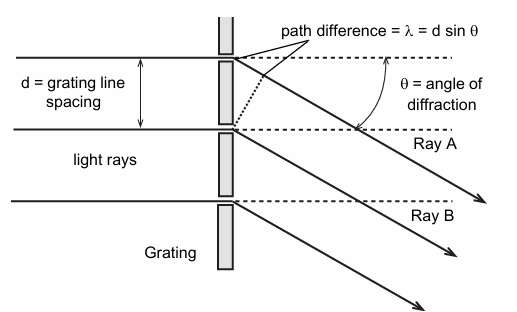
\includegraphics[width=0.5 \linewidth]{image1.png}
  \caption{Ray diagram for first order diffraction pattern}
  \label{image1}
\end{figure}

A diffraction grating is a transparent material on which a large number of equally spaced parallel lines have been ruled. The distance between these lines is called the grating line spacing, denoted by \(d\). When light strikes the grating, it is diffracted by these parallel lines. The diffracted light passes through the grating at all angles relative to the original light path. If the diffracted light rays from adjacent lines are in phase, an image of the light source is formed. This happens when the difference in path length between the light rays equals an integral multiple of the wavelength of the light.\\

The diffraction angle \( \theta \), at which light rays are diffracted by the grating, depends on the grating line spacing \(d\) and the wavelength \( \lambda \) of the light. The relationship is described by the diffraction equation:

\[
\lambda = d \sin \theta
\]

This equation allows for the determination of the wavelength \( \lambda \) when the diffraction angle \( \theta \) and the grating spacing \(d\) are known. In the \textbf{Figure~\ref{image1}}, the path difference for Ray A is one wavelength longer than the path difference for Ray B, illustrating the principle of constructive interference at the diffraction grating.\\

\begin{figure}[H]
  \centering
  \begin{subfigure}[b]{0.45\textwidth}
      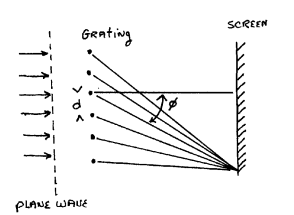
\includegraphics[width=\textwidth]{image2.png}
      \caption{Scattering From Many Grating Lines}
      \label{fig:grating_many_lines}
  \end{subfigure}
  \hfill
  \begin{subfigure}[b]{0.45\textwidth}
      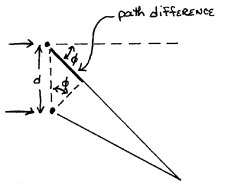
\includegraphics[width=\textwidth]{image3.png}
      \caption{Scattering From Two Grating Lines}
      \label{fig:grating_two_lines}
  \end{subfigure}
  \caption{Scattering diagrams showing the interaction of light waves with a diffraction grating.}
  \label{fig:grating_scattering}
\end{figure}

The diagrams in Figure~\ref{fig:grating_scattering} illustrate the scattering of light waves from a diffraction grating. Subfigure~\ref{fig:grating_many_lines} shows the scattering pattern generated by many grating lines, while Subfigure~\ref{fig:grating_two_lines} focuses on the scattering from two grating lines, highlighting the path difference responsible for constructive or destructive interference. These figures provide a foundational understanding of how light interacts with a grating to produce its characteristic diffraction pattern~\cite{cortland_lab_manual}.

\newpage
%%%%%%%%%%%%%%%%%%%%%%%%%%%%%%%%%%%%%%%%%
\phantomsection
\section*{\center METHODOLOGY}
\addcontentsline{toc}{section}{\large\numberline{3}METHODOLOGY} % Add numbered TOC entry
\label{sec:METHODOLOGY}
\begin{figure}[H]
  \centering
  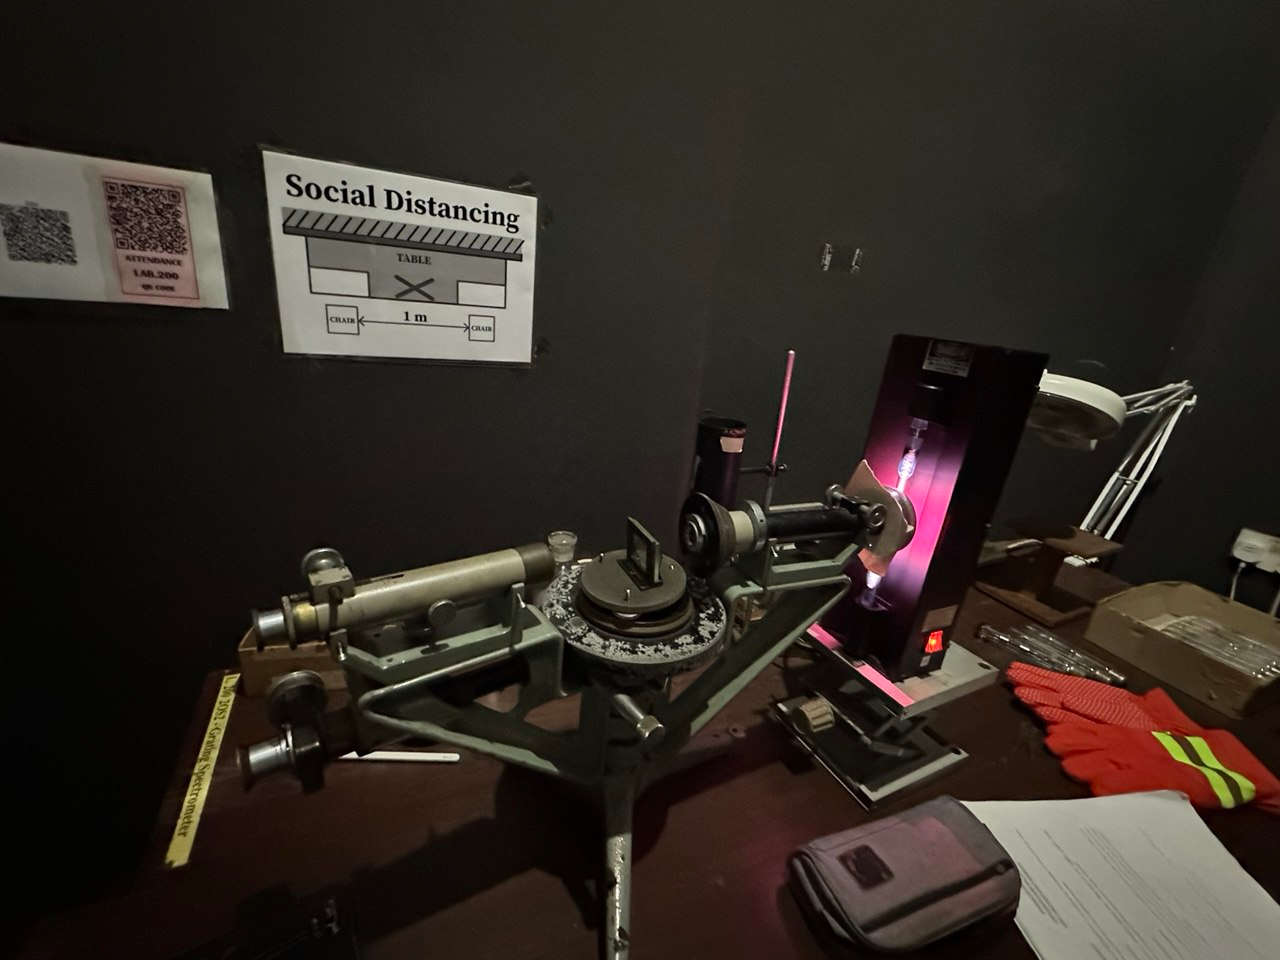
\includegraphics[width=0.7\textwidth]{experiment_setup_image.png}
  \caption{Experimental setup for the diffraction grating spectrometer. The setup includes the spectrometer (center), a light source (right) emitting the spectrum, and a telescope for observing and measuring diffraction angles. The diffraction grating is positioned between the collimator and the telescope to disperse the light into spectral lines.}
  \label{fig:experiment_setup}
\end{figure}

\quad The experiment involves using a diffraction grating spectrometer to measure the wavelengths of sodium, mercury, helium, cadmium, and hydrogen. The spectrometer is calibrated by first adjusting the telescope to focus on parallel rays and aligning the collimator for parallel light emission. A diffraction grating is then placed perpendicular to the axis of the collimator on the spectrometer table, ensuring proper alignment. The sodium lamp is switched on, and the telescope crosshairs are set on the central image to establish a zero-angle reference. The grating table is leveled, and the angles of diffraction maxima (\( \theta \)) on both sides of the light spectrum are measured using the Vernier scale. The measured angles are used in the grating equation:

\[
m \lambda = d \sin \theta,
\]

where \( d \) is the grating spacing, calculated as 

\[
d = \frac{1}{N},
\]

with \( N \) being the number of lines per millimeter on the grating. \( m \) is the order of the diffraction maxima, and \( \lambda \) is the wavelength. The procedure is repeated for mercury, helium, cadmium, and hydrogen discharge lamps. Data analysis includes computing the standard deviation of the wavelengths, comparing experimental wavelengths to standard values, and performing error analysis~\cite{usm_diffraction}.

\newpage
%%%%%%%%%%%%%%%%%%%%%%%%%%%%%%%%%%%%%%%%%%
\phantomsection
\section*{\center DATA ANALYSIS}
\addcontentsline{toc}{section}{\large\numberline{4}DATA ANALYSIS} % Add numbered TOC entry
\label{sec:DATA ANALYSIS}
% Content for the DATA ANALYSIS section goes here.
\textbf{All data, calculation and programming python code of the experments are attached in the Appendices.}\\

\quad \textbf{Table}~\ref{tab:spectral_data_elements} presents the spectral line data for various elements, including mercury (\(Hg\)), helium (\(He\)), cadmium (\(Cd\)), hydrogen (\(H_2\)), and sodium (\(Na\)).

\begin{table}[H]
  \centering
  \begin{tabular}{llllllllll}
  \toprule
  \textbf{Element} & \textbf{Color} & \(\boldsymbol{m}\) & \(\boldsymbol{\theta_L \text{ (deg)}}\) & \(\boldsymbol{\theta_R \text{ (deg)}}\) & \(\boldsymbol{\theta_L \text{ (rad)}}\) & \(\boldsymbol{\theta_R \text{ (rad)}}\) & \(\boldsymbol{\bar \theta \text{ (rad)}}\) \\
  \midrule
  Hg  & White        & 0 & 11°11'30" & 11°24'30"  & 0.195331 & 0.199113 & 0.197222 \\
  Hg  & Purple       & 1 & 25°54'30" & 26°13'0"   & 0.452186 & 0.457567 & 0.454876 \\
  Hg  & Green        & 1 & 29°47'30" & 30°8'30"   & 0.519963 & 0.526071 & 0.523017 \\
  Hg  & Yellow       & 1 & 30°52'50" & 31°14'0"   & 0.538967 & 0.545125 & 0.542046 \\
  Hg  & Purple       & 2 & 41°40'50" & 42°6'0"    & 0.727463 & 0.734784 & 0.731123 \\
  Hg  & Green        & 2 & 50°39'0"  & 50°56'30"  & 0.884009 & 0.889100 & 0.886555 \\
  Hg  & Yellow       & 2 & 53°19'0"  & 53°44'30"  & 0.930551 & 0.937969 & 0.934260 \\
  \hline
  He  & Orange       & 0 & 11°9'10"  & 11°22'40"  & 0.194653 & 0.198580 & 0.196616 \\
  He  & Blue       & 1 & 26°36'0"  & 26°54'0"   & 0.464258 & 0.469494 & 0.466876 \\
  He  & Cyan        & 1 & 28°20'0"  & 28°38'20"  & 0.494510 & 0.499843 & 0.497176 \\
  He  & Yellow       & 1 & 31°10'30" & 31°27'30"  & 0.544106 & 0.549051 & 0.546579 \\
  \hline
  Cd  & Cyan        & 0 & 11°17'30" & 11°32'0"   & 0.197077 & 0.201295 & 0.199186 \\
  Cd  & Blue    & 1 & 27°17'0"  & 27°38'10"  & 0.476184 & 0.482341 & 0.479263 \\
  Cd  & Light Blue   & 1 & 27°45'0"  & 28°4'10"   & 0.484329 & 0.489904 & 0.487117 \\
  Cd  & Green        & 1 & 28°47'10" & 29°8'10"   & 0.502412 & 0.508521 & 0.505467 \\
  \hline
  H2  & Reddish Pink & 0 & 11°7'20"  & 11°22'10"  & 0.194119 & 0.198434 & 0.196277 \\
  H2  & Blue    & 1 & 25°52'0"  & 26°10'40"  & 0.451458 & 0.456888 & 0.454173 \\
  H2  & Cyan   & 1 & 26°40'50" & 27°29'40"  & 0.465664 & 0.479869 & 0.472766 \\
  H2  & Red          & 1 & 33°39'20" & 34°49'40"  & 0.587400 & 0.607859 & 0.597630 \\
  \hline
  Na  & Orange       & 0 & 11°8'40"  & 11°23'10"  & 0.194507 & 0.198725 & 0.196616 \\
  Na  & Orange       & 1 & 31°11'0"  & 31°25'20"  & 0.544252 & 0.548421 & 0.546337 \\
  \bottomrule
  \end{tabular}
  \caption{Spectral Line Data for Various Elements with \(\bar \theta\) in Radians.}
  \label{tab:spectral_data_elements}
\end{table}

\newpage
The data in \textbf{Table}~\ref{tab:spectral_data_elements} highlight clear trends in the diffraction angles \(\bar{\theta}\) across multiple spectral lines for various elements. These angles increase with both the diffraction order (\(m\)) and the wavelength of the spectral line, which is consistent with the diffraction grating equation:

\[
d \sin \theta = m \lambda.
\]

For mercury (\(Hg\)), the yellow spectral line at first-order diffraction (\(m = 1\)) has a \(\bar{\theta}\) value of \(0.542046 \, \text{rad}\), while at second-order diffraction (\(m = 2\)), the angle increases to \(0.934260 \, \text{rad}\). This demonstrates that higher diffraction orders result in larger angular deviations. For helium (\(He\)), the angular measurements of the blue, cyan, and yellow lines show a systematic increase in \(\bar{\theta}\) with increasing wavelength.\\

Similar trends are observed for cadmium (\(Cd\)), where the first-order blue and green lines exhibit increasing values of \(\bar{\theta}\) at \(0.479263 \, \text{rad}\) and \(0.505467 \, \text{rad}\), respectively. For hydrogen (\(H_2\)), the red line has the largest angle among the observed spectral lines, with \(\bar{\theta} = 0.597630 \, \text{rad}\), reflecting its longer wavelength compared to the blue and cyan lines. The sodium (\(Na\)) spectral data further support these observations. The first-order orange line exhibits a \(\bar{\theta}\) value of \(0.546337 \, \text{rad}\), which is consistent with its longer wavelength. \\

Overall, the results validate the relationship between the diffraction angle and the wavelength of light. The consistency across elements and spectral lines demonstrates the reliability of the experimental setup and highlights the effectiveness of diffraction gratings for precise wavelength determination.

\newpage
\subsection*{Mercury}
\addcontentsline{toc}{subsection}{\large\numberline{4.1}Mercury} % Add numbered TOC entry
\label{sec:mercury}
% Hg
\textbf{Table}~\ref{tab:spectral_data_hg} presents the angular measurements, calculated diffraction angles and wavelengths for mercury’s spectral lines.
\begin{table}[H]
  \centering
  \begin{tabular}{lllllllll}
  \toprule
  \textbf{Color} & \(\boldsymbol{m}\) & \(\boldsymbol{\theta_L \text{ (deg)}}\) & \(\boldsymbol{\theta_R \text{ (deg)}}\) & \(\boldsymbol{\theta_L \text{ (rad)}}\) & \(\boldsymbol{\theta_R \text{ (rad)}}\) & \(\boldsymbol{\bar \theta \text{ (rad)}}\) & \(\boldsymbol{\theta \text{ (rad)}}\) & \(\boldsymbol{\lambda \text{ (nm)}}\) \\
  \midrule
  White  & 0 & 11°11'30" & 11°24'30" & 0.195331 & 0.199113 & 0.197222 & 0.000000 & 0 \\
  Purple & 1 & 25°54'30" & 26°13'0"  & 0.452186 & 0.457567 & 0.454877 & 0.257655 & 431.4845 \\
  Green  & 1 & 29°47'30" & 30°8'30"  & 0.519963 & 0.526071 & 0.523017 & 0.325795 & 542.4718 \\
  Yellow & 1 & 30°52'50" & 31°14'0"  & 0.538967 & 0.545125 & 0.542046 & 0.344824 & 572.3992 \\
  Purple & 2 & 41°40'50" & 42°6'0"   & 0.727463 & 0.734784 & 0.731124 & 0.533902 & 862.7308 \\
  Green  & 2 & 50°39'0"  & 50°56'30" & 0.883801 & 0.888333 & 0.886067 & 0.688845 & 1076.3605 \\
  Yellow & 2 & 53°19'0"  & 53°44'30" & 0.930109 & 0.937297 & 0.933703 & 0.736481 & 1137.3867 \\
  \bottomrule
  \end{tabular}
  \caption{Spectral Line Data for Mercury (Hg).}
  \label{tab:spectral_data_hg}
\end{table}

\quad Based on \textbf{Table}~\ref{tab:spectral_data_hg} the angular measurements and corresponding diffraction angles for various spectral lines observed in mercury light. The angles $\theta_L$ and $\theta_R$ were recorded symmetrically on both sides of the light spectrum. These angles were converted into radians, and the average diffraction angle $\bar{\theta}$ was calculated to determine the diffraction angle $\theta$ for each spectral line.\\

The angles \(\theta\) provided in \textbf{Table}~\ref{tab:spectral_data_hg} are calculated relative to the zeroth-order diffraction peak (\(m = 0\)), which serves as the reference point for all subsequent diffraction angles. The zeroth-order peak represents the central position where no diffraction occurs, corresponding to \(\theta = 0\). The angles \(\theta_L\) and \(\theta_R\) measured for higher orders (\(m = 1\) and \(m = 2\)) are absolute deviations from this reference point. By averaging these values, the mean diffraction angle \(\bar{\theta}\) accurately represents the position of the spectral lines relative to the zeroth order.\\

The results show that the diffraction angle $\theta$ increases with increasing wavelength $\lambda$, which is consistent with the diffraction grating equation \( d \sin\theta = m\lambda \). For instance, at \( m = 1 \), the diffraction angles for the purple, green and yellow lines are \textbf{0.257655 rad}, \textbf{0.325795 rad} and \textbf{0.344824 rad}, corresponding to wavelengths of \textbf{431.4845 nm}, \textbf{542.4718 nm} and \textbf{572.3992 nm}, respectively. For higher orders, such as \( m = 2 \), the angles increase further, as seen for the purple, green and yellow lines. This trend validates the theoretical expectation that longer wavelengths result in greater diffraction angles.\\

\textbf{Table}~\ref{tab:mercury_spectrum} compares the wavelengths calculated from the diffraction measurements with the theoretical (real) values of mercury’s spectral lines, along with their percentage difference.

\begin{table}[ht]
  \centering
  \begin{tabular}{lllll}
  \toprule
  \textbf{Color} & \(\boldsymbol{m}\) & \textbf{Calculated Wavelength (nm)} & \textbf{Real Wavelength (nm)} & \textbf{Percentage Difference (\%)} \\
  \midrule
  Purple & 1 & 431.4845 & 435.8328 & 1.00 \\
  Green  & 1 & 541.9718 & 546.0735 & 0.75 \\
  Yellow & 1 & 572.3992 & 567.7105 & 0.83 \\
  \bottomrule
  \end{tabular}
  \caption{Mercury spectrum data with calculated and real wavelengths, and their percentage differences.\cite{physicsSE_second_order_spectra}\cite{nist_mercury_spectrum}}
  \label{tab:mercury_spectrum}
  \end{table}

Based on \textbf{Table}~\ref{tab:mercury_spectrum}, a comparison between the calculated wavelengths obtained from the diffraction measurements and the theoretical (real) values of mercury's spectral lines, along with their percentage differences. For purple light, the calculated wavelength is \(\textbf{431.4845 \text{nm}}\), which is within \(1.00\%\) of the real value \(435.8328 \, \text{nm}\). For green light, the calculated wavelength is \(\textbf{541.9718\, \text{nm}}\), with a minor deviation of \(0.75\%\) from the theoretical value \(546.0735 \, \text{nm}\). Similarly, for yellow light, the calculated wavelength of \(\textbf{572.3992 \text{nm}}\) shows a small difference of \(0.83\%\) compared to the real value \(567.7105 \, \text{nm}\). 

\newpage
% He  
\subsection*{Helium}
\addcontentsline{toc}{subsection}{\large\numberline{4.2}Helium} % Add numbered TOC entry
\label{sec:helium}

\textbf{Table}~\ref{tab:spectral_data_he} presents the angular measurements, calculated diffraction angles, and wavelengths for helium’s spectral lines.
\begin{table}[H]
  \centering
  \begin{tabular}{lllllllll}
  \toprule
  \textbf{Color} & \(\boldsymbol{m}\) & \(\boldsymbol{\theta_L \text{ (deg)}}\) & \(\boldsymbol{\theta_R \text{ (deg)}}\) & \(\boldsymbol{\theta_L \text{ (rad)}}\) & \(\boldsymbol{\theta_R \text{ (rad)}}\) & \(\boldsymbol{\bar \theta \text{ (rad)}}\) & \(\boldsymbol{\theta \text{ (rad)}}\) & \(\boldsymbol{\lambda \text{ (nm)}}\) \\
  \midrule
  Orange & 0 & 11°9'10"  & 11°22'40"  & 0.194653 & 0.198580 & 0.196616 & 0.0000 & 0.0000 \\
  Blue & 1 & 26°36'0"  & 26°54'0"   & 0.464258 & 0.469494 & 0.466876 & 0.2703 & 452.0885 \\
  Cyan  & 1 & 28°20'0"  & 28°38'20"  & 0.494510 & 0.499843 & 0.497176 & 0.3006 & 501.3204 \\
  Yellow & 1 & 31°10'30" & 31°27'30"  & 0.544106 & 0.549051 & 0.546579 & 0.3500 & 580.5810 \\
  \bottomrule
  \end{tabular}
  \caption{Spectral Line Data for Helium (He).}
  \label{tab:spectral_data_he}
\end{table}
Based on \textbf{Table}~\ref{tab:spectral_data_he}, at \( m = 1 \), the diffraction angles for blue, cyan, and yellow light are \(\textbf{0.2703 \, \text{rad}}\), \(\textbf{0.3006 \, \text{rad}}\), and \(\textbf{0.3500 \, \text{rad}}\), corresponding to wavelengths of \(\textbf{452.0885 \, \text{nm}}\), \(\textbf{501.3204 \, \text{nm}}\), and \(\textbf{580.5810 \, \text{nm}}\), respectively. These values confirm that longer wavelengths result in larger diffraction angles, as expected.\\

\textbf{Table}~\ref{tab:Helium_spectrum} compares the wavelengths calculated from the diffraction measurements with the theoretical (real) values of helium's spectral lines, along with their percentage differences.

\begin{table}[ht]
  \centering
  \begin{tabular}{lllll}
  \toprule
  \textbf{Color} & \textbf{m} & \textbf{Calculated Wavelength (nm)} & \textbf{Real Wavelength (nm)} & \textbf{Percentage Difference (\%)} \\
  \midrule
  Blue   & 1 & 452.0885 & 447.1479 & 1.10 \\
  Cyan   & 1 & 501.3204 & 501.5678 & 0.05 \\
  Yellow & 1 & 580.5810 & 587.5615 & 1.19 \\
  \bottomrule
  \end{tabular}
  \caption{Helium spectrum data with calculated and real wavelengths, and their percentage differences.\cite{sciencephoto_helium_spectra}\cite{nist_helium_spectrum}}
  \label{tab:Helium_spectrum}
  \end{table}
  \quad Based on \textbf{Table}~\ref{tab:Helium_spectrum}, the calculated wavelengths closely match the real (theoretical) values, with small percentage differences observed. For blue light, the calculated wavelength of \(\textbf{452.0885\, \text{nm}}\) deviates by \(1.10\%\) from the real value \(447.1479 \, \text{nm}\). For cyan light, the calculated wavelength of \(\textbf{501.3204\, \text{nm}}\) shows excellent agreement with the theoretical value \(501.5678 \, \text{nm}\), with a negligible percentage difference of \(0.05\%\). Similarly, the yellow light has a calculated wavelength of \(\textbf{580.5810\, \text{nm}}\), which deviates by \(1.19\%\) from the real value \(587.5615 \, \text{nm}\).

\newpage
%Cd
\subsection*{Cadmium}
\addcontentsline{toc}{subsection}{\large\numberline{4.3}Cadmium} % Add numbered TOC entry
\label{sec:cadmium}

\textbf{Table}~\ref{tab:spectral_data_cd} presents the angular measurements, calculated diffraction angles, and wavelengths for cadmium’s spectral lines.

\begin{table}[H]
  \centering
  \begin{tabular}{llllllllll}
  \toprule
  \textbf{Color} & \(\boldsymbol{m}\) & \(\boldsymbol{\theta_L \text{ (deg)}}\) & \(\boldsymbol{\theta_R \text{ (deg)}}\) & \(\boldsymbol{\theta_L \text{ (rad)}}\) & \(\boldsymbol{\theta_R \text{ (rad)}}\) & \(\boldsymbol{\bar \theta \text{ (rad)}}\) & \(\boldsymbol{\theta \text{ (rad)}}\) & \(\boldsymbol{\lambda \text{ (nm)}}\) \\
  \midrule
  Cyan      & 0 & 11°17'30" & 11°32'0"  & 0.197077 & 0.201295 & 0.199186 & 0.0000 & 0.0000 \\
  Blue  & 1 & 27°17'0"  & 27°38'10" & 0.476184 & 0.482341 & 0.479263 & 0.2801 & 468.0873 \\
  Light Blue & 1 & 27°45'0"  & 28°4'10"  & 0.484329 & 0.489904 & 0.487117 & 0.2879 & 480.8539 \\
  Green      & 1 & 28°47'10" & 29°8'10"  & 0.502412 & 0.508521 & 0.505467 & 0.3063 & 510.5651 \\
  \bottomrule
  \end{tabular}
  \caption{Spectral Line Data for Cadmium (Cd).}
  \label{tab:spectral_data_cd}
\end{table}

\quad Based on \textbf{Table}~\ref{tab:spectral_data_cd}, at \(m = 1\), the diffraction angles for blue, light blue, and green spectral lines are \(\textbf{0.2801 \, \text{rad}}\), \(\textbf{0.2879 \, \text{rad}}\), and \(\textbf{0.3063 \, \text{rad}}\), corresponding to wavelengths of \(\textbf{468.0873 \, \text{nm}}\), \(\textbf{480.8539 \, \text{nm}}\), and \(\textbf{510.5651 \, \text{nm}}\), respectively. This observation aligns with the theoretical relationship where the diffraction angle increases with increasing wavelength.\\

\textbf{Table}~\ref{tab:Cadmium_spectrum} compares the wavelengths calculated from the diffraction measurements with the theoretical (real) values of cadmium's spectral lines, along with their percentage differences.

\begin{table}[ht]
  \centering
  \begin{tabular}{lllll}
  \toprule
  \textbf{Color} & \textbf{m} & \textbf{Calculated Wavelength (nm)} & \textbf{Real Wavelength (nm)} & \textbf{Percentage Difference (\%)} \\
  \midrule
  Blue       & 1 & 468.0873 & 467.8149 & 0.06 \\
  Light Blue & 1 & 480.8539 & 479.9912 & 0.18 \\
  Green      & 1 & 510.5651 & 508.5822 & 0.39 \\
  \bottomrule
  \end{tabular}
  \caption{Cadmium spectrum data with calculated and real wavelengths, and their percentage differences.\cite{sciencephoto_cadmium_spectrum}\cite{nist_cadmium_spectrum}}
  \label{tab:Cadmium_spectrum}
  \end{table}

\quad Based on \textbf{Table}~\ref{tab:Cadmium_spectrum}, the calculated wavelengths closely match the real (theoretical) values of cadmium’s spectral lines, with small percentage differences observed. For blue light, the calculated wavelength of \(\textbf{468.0873 \, \text{nm}}\) deviates by only \(0.06\%\) from the real value \(467.8149 \, \text{nm}\). Similarly, for light blue light, the calculated wavelength of \(\textbf{480.8539 \, \text{nm}}\) has a small difference of \(0.18\%\) compared to the real value \(479.9912 \, \text{nm}\). The green light shows a calculated wavelength of \(\textbf{510.5651 \, \text{nm}}\), with a deviation of \(0.39\%\) from the real value \(508.5822 \, \text{nm}\).

\newpage
%H2
\subsection*{Hydrogen}
\addcontentsline{toc}{subsection}{\large\numberline{4.4}Hydrogen} % Add numbered TOC entry
\label{sec:hydrogen}

\textbf{Table}~\ref{tab:spectral_data_h2} presents the angular measurements, calculated diffraction angles, and wavelengths for hydrogen's spectral lines.
\begin{table}[H]
  \centering
  \begin{tabular}{llllllllll}
  \toprule
  \textbf{Color} & \(\boldsymbol{m}\) & \(\boldsymbol{\theta_L \text{ (deg)}}\) & \(\boldsymbol{\theta_R \text{ (deg)}}\) & \(\boldsymbol{\theta_L \text{ (rad)}}\) & \(\boldsymbol{\theta_R \text{ (rad)}}\) & \(\boldsymbol{\bar \theta \text{ (rad)}}\) & \(\boldsymbol{\theta \text{ (rad)}}\) & \(\boldsymbol{\lambda \text{ (nm)}}\) \\
  \midrule
  Reddish Pink & 0 & 11°7'20"  & 11°22'10"  & 0.194119 & 0.198434 & 0.196277 & 0.0000 & 0.0000 \\
  Blue    & 1 & 25°52'0"  & 26°10'40"  & 0.451458 & 0.456888 & 0.454173 & 0.2579 & 431.8801 \\
  Cyan   & 1 & 26°40'50" & 27°29'40"  & 0.465664 & 0.479869 & 0.472766 & 0.2765 & 462.2460 \\
  Red          & 1 & 33°39'20" & 34°49'40"  & 0.587400 & 0.607859 & 0.597630 & 0.4014 & 661.5247 \\
  \bottomrule
  \end{tabular}
  \caption{Spectral Line Data for Hydrogen (\(H_2\)).}
  \label{tab:spectral_data_h2}
\end{table}

\quad Based on \textbf{Table}~\ref{tab:spectral_data_h2}, at \(m = 1\), the diffraction angles for blue, cyan, and red spectral lines are \(\textbf{0.2579 \, \text{rad}}\), \(\textbf{0.2765 \, \text{rad}}\), and \(\textbf{0.4014 \, \text{rad}}\), corresponding to wavelengths of \(\textbf{431.8801 \, \text{nm}}\), \(\textbf{462.2460 \, \text{nm}}\), and \(\textbf{661.5247 \, \text{nm}}\), respectively. These results clearly show that longer wavelengths correspond to larger diffraction angles, which is consistent with theoretical predictions.\\

\textbf{Table}~\ref{tab:Hydrogen_spectrum} compares the calculated wavelengths with the theoretical (real) values of hydrogen's spectral lines and their percentage differences.

\begin{table}[H]
\centering
\begin{tabular}{lllll}
\toprule
\textbf{Color} & \textbf{m} & \textbf{Calculated Wavelength (nm)} & \textbf{Real Wavelength (nm)} & \textbf{Percentage Difference (\%)} \\
\midrule
Blue & 1 & 431.8801 & 434.0462 & 0.50 \\
Cyan & 1 & 462.2460 & 486.1362 & 4.91 \\
Red  & 1 & 661.5247 & 656.2852 & 0.80 \\
\bottomrule
\end{tabular}
\caption{Hydrogen spectrum data with calculated and real wavelengths, and their percentage differences.\cite{utexas_hydrogen_spectra}\cite{nist_hydrogen_spectrum}}
\label{tab:Hydrogen_spectrum}
\end{table}

\quad Based on \textbf{Table}~\ref{tab:Hydrogen_spectrum}, the calculated wavelengths are compared with the theoretical values for hydrogen's spectral lines. The results show that the blue light has a calculated wavelength of \(\textbf{431.8801 \, \text{nm}}\), which deviates by \(0.50\%\) from the real value of \(434.0462 \, \text{nm}\). For cyan light, the calculated wavelength is \(\textbf{462.2460 \, \text{nm}}\), with a larger percentage difference of \(4.91\%\) compared to the theoretical value \(486.1362 \, \text{nm}\). The red light has a calculated wavelength of \(\textbf{661.5247 \, \text{nm}}\), showing a small deviation of \(0.80\%\) from the real value \(656.2852 \, \text{nm}\).
\newpage
%Na
\subsection*{Sodium}
\addcontentsline{toc}{subsection}{\large\numberline{4.5}Sodium} % Add numbered TOC entry
\label{sec:sodium}

\textbf{Table}~\ref{tab:spectral_data_na} presents the angular measurements, calculated diffraction angles, and wavelengths for sodium’s spectral lines.\\

\begin{table}[H]
  \centering
  \begin{tabular}{llllllllll}
  \toprule
  \textbf{Color} & \(\boldsymbol{m}\) & \(\boldsymbol{\theta_L \text{ (deg)}}\) & \(\boldsymbol{\theta_R \text{ (deg)}}\) & \(\boldsymbol{\theta_L \text{ (rad)}}\) & \(\boldsymbol{\theta_R \text{ (rad)}}\) & \(\boldsymbol{\bar \theta \text{ (rad)}}\) & \(\boldsymbol{\theta \text{ (rad)}}\) & \(\boldsymbol{\lambda \text{ (nm)}}\) \\
  \midrule
  Orange & 0 & 11°8'40"  & 11°23'10"  & 0.194507 & 0.198725 & 0.196616 & 0.00000 & 0.0000 \\
  Orange & 1 & 31°11'0"  & 31°25'20"  & 0.544252 & 0.548421 & 0.546337 & 0.34972 & 580.1954 \\
  \bottomrule
  \end{tabular}
  \caption{Spectral Line Data for Sodium (\(Na\)).}
  \label{tab:spectral_data_na}
\end{table}

\quad Based on \textbf{Table}~\ref{tab:spectral_data_na}, at \(m = 1\), the diffraction angle for the orange line is \(\textbf{0.34972 \, \text{rad}}\), corresponding to a calculated wavelength of \(\textbf{580.1954 \, \text{nm}}\). This observation confirms the relationship where longer wavelengths are associated with larger diffraction angles.\\

\textbf{Table}~\ref{tab:Sodium_spectrum} compares the calculated wavelength with the theoretical (real) value of sodium’s spectral line and the percentage difference.\\

\begin{table}[ht]
\centering
\begin{tabular}{lllll}
\toprule
\textbf{Color} & \textbf{m} & \textbf{Calculated Wavelength (nm)} & \textbf{Real Wavelength (nm)} & \textbf{Percentage Difference (\%)} \\
\midrule
Orange & 1 & 580.1954 & 588.995 & 1.49 \\
\bottomrule
\end{tabular}
\caption{Sodium spectrum data with calculated and real wavelengths, and their percentage differences.\cite{lighting_gallery_sodium_spectrum}\cite{nist_sodium_spectrum}}
\label{tab:Sodium_spectrum}
\end{table}

\qquad Based on \textbf{Table}~\ref{tab:Sodium_spectrum}, the calculated wavelength for the orange line is \(\textbf{580.1954 \, \text{nm}}\), which deviates by \(1.49\%\) from the real wavelength of \(588.995 \, \text{nm}\). This small discrepancy can be attributed to minor uncertainties in the angular measurements, instrumental resolution, or imperfections in the diffraction grating. Despite the minor difference, the experimental results closely align with the theoretical value, validating the diffraction grating method as an accurate tool for measuring spectral line wavelengths.

%%%%%%%%%%%%%%%%%%%%%%%%%%%%%%%%%%%%%%%%%
\phantomsection
\section*{\center DISCUSSION}
\addcontentsline{toc}{section}{\large\numberline{5}DISCUSSION} % Add numbered TOC entry
\label{sec:DISCUSSION}
% Content for the DISCUSSION section goes here.

\qquad In this experiment, a diffraction grating spectrometer was employed to measure the wavelengths of light emitted by sodium, mercury, helium, cadmium, and hydrogen. The grating equation, \( \lambda = m \lambda \), was utilized to calculate the wavelengths, where \( \theta \) is the diffraction angle, \( d \) is the grating spacing, and \( m \) represents the diffraction order. This equation provided the foundation for analyzing the diffraction patterns observed.\\

In the case of \textbf{mercury (\(Hg\))}, the first-order spectral lines for purple, green, and yellow light were measured. The calculated wavelengths were \(431.4845 \, \text{nm}\), \(541.9718 \, \text{nm}\), and \(572.3992 \, \text{nm}\), compared to their respective theoretical values of \(435.8328 \, \text{nm}\), \(546.0735 \, \text{nm}\), and \(567.7105 \, \text{nm}\). The percentage differences were \(1.00\%\), \(0.75\%\), and \(0.83\%\), respectively. These results confirm the experiment's precision, with minor discrepancies arising from small angular reading errors.\\

For \textbf{helium (\(He\))}, the blue, cyan, and yellow spectral lines were analyzed. The calculated wavelengths were \(452.0885 \, \text{nm}\), \(501.3204 \, \text{nm}\), and \(580.5810 \, \text{nm}\), compared to their theoretical values of \(447.1479 \, \text{nm}\), \(501.5678 \, \text{nm}\), and \(587.5615 \, \text{nm}\). The percentage differences were \(1.10\%\), \(0.05\%\), and \(1.19\%\), respectively. The cyan line showed an exceptional agreement with the theoretical value, confirming the diffraction grating's reliability, while minor deviations for the other lines reflected systematic measurement uncertainties.\\

For \textbf{cadmium (\(Cd\))}, the blue, light blue, and green lines were observed at \(m=1\). The calculated wavelengths were \(468.0873 \, \text{nm}\), \(480.8539 \, \text{nm}\), and \(510.5651 \, \text{nm}\), compared to their theoretical values of \(467.8149 \, \text{nm}\), \(479.9912 \, \text{nm}\), and \(508.5822 \, \text{nm}\). The corresponding percentage differences were \(0.06\%\), \(0.18\%\), and \(0.39\%\), indicating high precision in the measurements.\\

For \textbf{hydrogen (\(H_2\))}, the blue, cyan, and red spectral lines were analyzed. The calculated wavelengths were \(431.8801 \, \text{nm}\), \(462.2460 \, \text{nm}\), and \(661.5247 \, \text{nm}\), with theoretical values of \(434.0462 \, \text{nm}\), \(486.1362 \, \text{nm}\), and \(656.2852 \, \text{nm}\), respectively. The percentage differences were \(0.50\%\) for the blue line, \(4.91\%\) for the cyan line, and \(0.80\%\) for the red line. The larger deviation for the cyan line likely resulted from difficulties in observing faint spectral lines and alignment errors.\\

For \textbf{sodium (\(Na\))}, the measured orange spectral line at \(m=1\) produced a calculated wavelength of \(580.1954 \, \text{nm}\), compared to the theoretical value of \(588.995 \, \text{nm}\), yielding a percentage difference of \(1.49\%\). This small deviation reflects the method's accuracy, with slight errors attributed to alignment issues and instrumental resolution.\\

Various sources of error were identified during the experiment. Instrumental factors included potential imperfections or damage to the diffraction grating, which could affect the uniformity of line spacing and introduce inaccuracies in measured angles. The presence of dust on the diffraction grating's lens may have caused unwanted reflections of light, interfering with the clarity and precision of the diffraction pattern. Misalignment of the collimator and telescope also posed a risk to angle measurements, impacting the accuracy of the calculated wavelengths. The inability to adjust the focus of the spectrometer to the actual position of the spectral lines could have further affected the accuracy of the angular readings, leading to minor discrepancies between the calculated and theoretical wavelengths. The low intensity of the light sources contributed to the dimness of the observed spectral lines, making it difficult to clearly identify the boundaries of the light spectrum. This limitation could have introduced errors in measuring the diffraction angles. Environmental influences, such as temperature fluctuations and air currents, altered the refractive index, potentially affecting the diffraction patterns. Human limitations, particularly the eye's reduced sensitivity to dim spectral lines in the red and violet regions, further complicated precise observations.\\

To address these challenges, several improvements were adopted. Cleaning the dust on diffraction grating glass by using alcohol and cotton swab. Regular calibration of the spectrometer using light sources with known wavelengths ensured systematic errors were identified and corrected. Experiments were conducted in controlled environments to minimize external disturbances like temperature variations and air currents. Sensitive detection equipment, such as photomultiplier tubes or CCDs (Charge-coupled Device), enhanced the visibility of dim spectral lines, compensating for human limitations. Increasing the number of slits in the diffraction grating was another effective strategy, as it sharpened the diffraction maxima and improved the resolution and precision of wavelength measurements.\\

\newpage
%%%%%%%%%%%%%%%%%%%%%%%%%%%%%%%%%%%%%%%%%%
\phantomsection
\section*{\center CONCLUSION}
\addcontentsline{toc}{section}{\large\numberline{6}CONCLUSION} % Add numbered TOC entry
\label{sec:CONCLUSION}
% Content for the CONCLUSION section goes here.
\noindent
\qquad For the Mercury spectrum, the wavelengths are \(431.48 \, \text{nm}\) for purple, \(541.97 \, \text{nm}\) for green, and \(572.40 \, \text{nm}\) for yellow. \\

\quad For the Helium spectrum, the wavelengths are \(452.09 \, \text{nm}\) for blue, \(501.32 \, \text{nm}\) for cyan, and \(580.58 \, \text{nm}\) for yellow. \\

\quad For the Cadmium spectrum, the wavelengths are \(468.09 \, \text{nm}\) for blue, \(480.85 \, \text{nm}\) for light blue, and \(510.57 \, \text{nm}\) for green. \\

\quad For the Hydrogen spectrum, the wavelengths are \(431.88 \, \text{nm}\) for blue, \(462.25 \, \text{nm}\) for cyan, and \(661.52 \, \text{nm}\) for red. \\

\quad For the Sodium spectrum, the wavelengths are \(580.20 \, \text{nm}\) for orange. \\

\newpage
%%%%%%%%%%%%%%%%%%%%%%%%%%%%%%%%%%%%%%%%%%
\phantomsection
\section*{\center REFERENCES}
\addcontentsline{toc}{section}{\large REFERENCES} % Add numbered TOC entry
\label{sec:REFERENCES}

\printbibliography[heading=none]

\newpage
%%%%%%%%%%%%%%%%%%%%%%%%%%%%%%%%%%%%%%%%%%
\phantomsection
\section*{\center APPENDICES}
\addcontentsline{toc}{section}{\large APPENDICES} % Add numbered TOC entry
\label{sec:APPENDICES}
%
\subsection*{Data}
\addcontentsline{toc}{subsection}{\large\numberline{}Data} % Add numbered TOC entry
\begin{lstlisting}[language=Python]
  import math
  import pandas as pd
  
  # Function to convert degrees, minutes, and seconds to radians
  def dms_to_radians(degrees, minutes, seconds):
      total_degrees = degrees + minutes / 60 + seconds / 3600
      return math.radians(total_degrees)
  
  # Data for the table
  data = [
      ["Hg", "White", 0, (11, 11, 30), (11, 24, 30)],
      ["Hg", "Purple", 1, (25, 54, 30), (26, 13, 0)],
      ["Hg", "Green", 1, (29, 47, 30), (30, 8, 30)],
      ["Hg", "Yellow", 1, (30, 52, 50), (31, 14, 0)],
      ["Hg", "Purple", 2, (41, 40, 50), (42, 6, 0)],
      ["Hg", "Green", 2, (50, 39, 0), (50, 56, 30)],
      ["Hg", "Yellow", 2, (53, 19, 0), (53, 44, 30)],
      ["He", "Orange", 0, (11, 9, 10), (11, 22, 40)],
      ["He", "Blue", 1, (26, 36, 0), (26, 54, 0)],
      ["He", "Cyan", 1, (28, 20, 0), (28, 38, 20)],
      ["He", "Yellow", 1, (31, 10, 30), (31, 27, 30)],
      ["Cd", "Cyan", 0, (11, 17, 30), (11, 32, 0)],
      ["Cd", "Blue", 1, (27, 17, 0), (27, 38, 10)],
      ["Cd", "Light Blue", 1, (27, 45, 0), (28, 4, 10)],
      ["Cd", "Green", 1, (28, 47, 10), (29, 8, 10)],
      ["H2", "Reddish Pink", 0, (11, 7, 20), (11, 22, 10)],
      ["H2", "Blue", 1, (25, 52, 0), (26, 10, 40)],
      ["H2", "Cyan", 1, (26, 40, 50), (27, 29, 40)],
      ["H2", "Red", 1, (33, 39, 20), (34, 49, 40)],
      ["Na", "Orange", 0, (11, 8, 40), (11, 23, 10)],
      ["Na", "Orange", 1, (31, 11, 0), (31, 25, 20)],
  ]
  
  # Process the data
  processed_data = []
  for element, color, m, theta_L, theta_R in data:
      theta_L_rad = dms_to_radians(*theta_L)
      theta_R_rad = dms_to_radians(*theta_R)
      delta_theta_rad = (theta_L_rad + theta_R_rad) / 2
      processed_data.append([element, color, m, theta_L, theta_R, theta_L_rad, theta_R_rad, delta_theta_rad])
  
  # Create a DataFrame
  columns = [
      "Element", "Color", "m", "Theta_L (deg)", "Theta_R (deg)", "Theta_L (rad)", "Theta_R (rad)", "Delta Theta (rad)"
  ]
  df = pd.DataFrame(processed_data, columns=columns)
  
  # Display the DataFrame
  print(df)
  
\end{lstlisting}
\newpage
\subsection*{Output}
\begin{lstlisting}[language=Python]
  Element         Color  m Theta_L (deg) Theta_R (deg)  Theta_L (rad)  \
  0       Hg         White  0  (11, 11, 30)  (11, 24, 30)       0.195331   
  1       Hg        Purple  1  (25, 54, 30)   (26, 13, 0)       0.452186   
  2       Hg         Green  1  (29, 47, 30)   (30, 8, 30)       0.519963   
  3       Hg        Yellow  1  (30, 52, 50)   (31, 14, 0)       0.538967   
  4       Hg        Purple  2  (41, 40, 50)    (42, 6, 0)       0.727463   
  5       Hg         Green  2   (50, 39, 0)  (50, 56, 30)       0.884009   
  6       Hg        Yellow  2   (53, 19, 0)  (53, 44, 30)       0.930551   
  7       He        Orange  0   (11, 9, 10)  (11, 22, 40)       0.194653   
  8       He          Blue  1   (26, 36, 0)   (26, 54, 0)       0.464258   
  9       He          Cyan  1   (28, 20, 0)  (28, 38, 20)       0.494510   
  10      He        Yellow  1  (31, 10, 30)  (31, 27, 30)       0.544106   
  11      Cd          Cyan  0  (11, 17, 30)   (11, 32, 0)       0.197077   
  12      Cd          Blue  1   (27, 17, 0)  (27, 38, 10)       0.476184   
  13      Cd    Light Blue  1   (27, 45, 0)   (28, 4, 10)       0.484329   
  14      Cd         Green  1  (28, 47, 10)   (29, 8, 10)       0.502412   
  15      H2  Reddish Pink  0   (11, 7, 20)  (11, 22, 10)       0.194119   
  16      H2          Blue  1   (25, 52, 0)  (26, 10, 40)       0.451458   
  17      H2          Cyan  1  (26, 40, 50)  (27, 29, 40)       0.465664   
  18      H2           Red  1  (33, 39, 20)  (34, 49, 40)       0.587400   
  19      Na        Orange  0   (11, 8, 40)  (11, 23, 10)       0.194507   
  20      Na        Orange  1   (31, 11, 0)  (31, 25, 20)       0.544252   
  
      Theta_R (rad)  Delta Theta (rad)  
  0        0.199113           0.197222  
  1        0.457567           0.454876  
  2        0.526071           0.523017  
  3        0.545125           0.542046  
  4        0.734784           0.731123  
  5        0.889100           0.886555  
  6        0.937969           0.934260  
  7        0.198580           0.196616  
  8        0.469494           0.466876  
  9        0.499843           0.497176  
  10       0.549051           0.546579  
  11       0.201295           0.199186  
  12       0.482341           0.479263  
  13       0.489904           0.487117  
  14       0.508521           0.505467  
  15       0.198434           0.196277  
  16       0.456888           0.454173  
  17       0.479869           0.472766  
  18       0.607859           0.597630  
  19       0.198725           0.196616  
  20       0.548421           0.546337
\end{lstlisting}
\newpage
%
\subsection*{Mercury}
\addcontentsline{toc}{subsection}{\large\numberline{}Mercury} % Add numbered TOC entry
\begin{lstlisting}[language=Python]
  import math
  import pandas as pd
  
  # Data for the table
  data = [
      ["White", 0, (11, 11, 30), (11, 24, 30), 0.195331, 0.199113, 0.197222],
      ["Purple", 1, (25, 54, 30), (26, 13, 0), 0.452186, 0.457567, 0.454877],
      ["Green", 1, (29, 47, 30), (30, 8, 30), 0.519963, 0.526071, 0.523017],
      ["Yellow", 1, (30, 52, 50), (31, 14, 0), 0.538967, 0.545125, 0.542046],
      ["Purple", 2, (41, 40, 50), (42, 6, 0), 0.727463, 0.734784, 0.731124],
      ["Green", 2, (50, 39, 0), (50, 56, 30), 0.883801, 0.888333, 0.886067],
      ["Yellow", 2, (53, 19, 0), (53, 44, 30), 0.930109, 0.937297, 0.933703],
  ]
  
  # Create a DataFrame
  columns = [
      "Color", "m", "Theta_L (deg)", "Theta_R (deg)", "Theta_L (rad)", "Theta_R (rad)", "Delta Theta (rad)"
  ]
  df = pd.DataFrame(data, columns=columns)
  
  # Extract Delta Theta for m = 0
  delta_theta_m0 = df[df["m"] == 0]["Delta Theta (rad)"].iloc[0]
  
  # Calculate theta for each color
  df["Theta (rad)"] = df["Delta Theta (rad)"] - delta_theta_m0
  
  # Grating spacing in nanometers
  d_inch = 1 / 15000  # d in inches
  d_meter = d_inch * 0.0254  # Convert d to meters
  d_nm = d_meter * 1e9  # Convert d to nanometers
  
  # Calculate d * sin(Theta) in nanometers
  df["d sin(Theta) (nm)"] = (d_nm * df["Theta (rad)"].apply(math.sin)).round(4)
  
  # Display the updated DataFrame
  print(df)
\end{lstlisting}
\newpage
\subsection*{Output}
\begin{lstlisting}[language=Python]
  Color  m Theta_L (deg) Theta_R (deg)  Theta_L (rad)  Theta_R (rad)  \
  0   White  0  (11, 11, 30)  (11, 24, 30)       0.195331       0.199113   
  1  Purple  1  (25, 54, 30)   (26, 13, 0)       0.452186       0.457567   
  2   Green  1  (29, 47, 30)   (30, 8, 30)       0.519963       0.526071   
  3  Yellow  1  (30, 52, 50)   (31, 14, 0)       0.538967       0.545125   
  4  Purple  2  (41, 40, 50)    (42, 6, 0)       0.727463       0.734784   
  5   Green  2   (50, 39, 0)  (50, 56, 30)       0.883801       0.888333   
  6  Yellow  2   (53, 19, 0)  (53, 44, 30)       0.930109       0.937297   
  
     Delta Theta (rad)  Theta (rad)  d sin(Theta) (nm)  
  0           0.197222     0.000000             0.0000  
  1           0.454877     0.257655           431.4845  
  2           0.523017     0.325795           541.9718  
  3           0.542046     0.344824           572.3992  
  4           0.731124     0.533902           861.7308  
  5           0.886067     0.688845          1076.3605  
  6           0.933703     0.736481          1137.3867
\end{lstlisting}

\newpage
%
\subsection*{Mercury percentage difference}
\addcontentsline{toc}{subsection}{\large\numberline{}Mercury percentage difference} % Add numbered TOC entry
\begin{lstlisting}[language=Python]
  import pandas as pd

  # Provided data for m = 1
  data = {
      "Color": ["Purple", "Green", "Yellow"],
      "m": [1, 1, 1],
      "Calculated Wavelength (nm)": [431.4845, 541.9718, 572.3992],
  }
  
  # Add the real wavelength values provided by the user for m = 1
  real_values = [435.8328, 546.0735, 567.7105]  # Replace with your actual values
  data["Real Wavelength (nm)"] = real_values
  
  # Create a DataFrame
  df = pd.DataFrame(data)
  
  # Calculate the percentage difference
  df["Percentage Difference (%)"] = (
      abs(df["Calculated Wavelength (nm)"] - df["Real Wavelength (nm)"]) / df["Real Wavelength (nm)"] * 100
  ).round(2)
  
  # Show only the required columns
  result_df = df[["Color", "m", "Calculated Wavelength (nm)", "Real Wavelength (nm)", "Percentage Difference (%)"]]
  
  # Display the result DataFrame
  print(result_df)
  
\end{lstlisting}
\newpage
\subsection*{Output}
\begin{lstlisting}[language=Python]
  Color  m  Calculated Wavelength (nm)  Real Wavelength (nm)  \
  0  Purple  1                    431.4845              435.8328   
  1   Green  1                    541.9718              546.0735   
  2  Yellow  1                    572.3992              567.7105   
  
     Percentage Difference (%)  
  0                       1.00  
  1                       0.75  
  2                       0.83
\end{lstlisting}

\newpage
%
\subsection*{Helium}
\addcontentsline{toc}{subsection}{\large\numberline{}Helium} % Add numbered TOC entry
\begin{lstlisting}[language=Python]
  import math
  import pandas as pd
  
  # Function to convert degrees, minutes, and seconds to radians
  def dms_to_radians(degrees, minutes, seconds):
      total_degrees = degrees + minutes / 60 + seconds / 3600
      return math.radians(total_degrees)
  
  # Data for the table
  data = [
      ["Orange", 0, (11, 9, 10), (11, 22, 40)],
      ["Blue", 1, (26, 36, 0), (26, 54, 0)],
      ["Cyan", 1, (28, 20, 0), (28, 38, 20)],
      ["Yellow", 1, (31, 10, 30), (31, 27, 30)],
  ]
  
  # Process the data
  processed_data = []
  for color, m, theta_L_dms, theta_R_dms in data:
      theta_L_rad = dms_to_radians(*theta_L_dms)
      theta_R_rad = dms_to_radians(*theta_R_dms)
      delta_theta_rad = (theta_L_rad + theta_R_rad) / 2
      processed_data.append([color, m, theta_L_dms, theta_R_dms, theta_L_rad, theta_R_rad, delta_theta_rad])
  
  # Create a DataFrame
  columns = [
      "Color", "m", "Theta_L (deg)", "Theta_R (deg)", "Theta_L (rad)", "Theta_R (rad)", "Delta Theta (rad)"
  ]
  df = pd.DataFrame(processed_data, columns=columns)
  
  # Extract Delta Theta for m = 0
  delta_theta_m0 = df[df["m"] == 0]["Delta Theta (rad)"].iloc[0]
  
  # Calculate theta for each color
  df["Theta (rad)"] = df["Delta Theta (rad)"] - delta_theta_m0
  
  # Grating spacing in nanometers
  d_inch = 1 / 15000  # d in inches
  d_meter = d_inch * 0.0254  # Convert d to meters
  d_nm = d_meter * 1e9  # Convert d to nanometers
  
  # Calculate d * sin(Theta) in nanometers
  df["d sin(Theta) (nm)"] = (d_nm * df["Theta (rad)"].apply(math.sin)).round(4)
  
  # Display the updated DataFrame
  print(df)
\end{lstlisting}
\subsection*{Output}
\begin{lstlisting}[language=Python]
  Color  m Theta_L (deg) Theta_R (deg)  Theta_L (rad)  Theta_R (rad)  \
  0  Orange  0   (11, 9, 10)  (11, 22, 40)       0.194653       0.198580   
  1    Blue  1   (26, 36, 0)   (26, 54, 0)       0.464258       0.469494   
  2    Cyan  1   (28, 20, 0)  (28, 38, 20)       0.494510       0.499843   
  3  Yellow  1  (31, 10, 30)  (31, 27, 30)       0.544106       0.549051   
  
     Delta Theta (rad)  Theta (rad)  d sin(Theta) (nm)  
  0           0.196616     0.000000             0.0000  
  1           0.466876     0.270259           452.0885  
  2           0.497176     0.300560           501.3204  
  3           0.546579     0.349963           580.5810
\end{lstlisting}

\newpage
%
\subsection*{Helium percentage difference}
\addcontentsline{toc}{subsection}{\large\numberline{}Helium percentage difference} % Add numbered TOC entry
\begin{lstlisting}[language=Python]
  import pandas as pd

  # Provided data for m = 1
  data = {
      "Color": ["Blue", "Cyan", "Yellow"],
      "m": [1, 1, 1],
      "Calculated Wavelength (nm)": [452.0885,501.3204,580.5810]
  }
  
  # Real wavelength values for m = 1
  real_values = [447.1479,501.5678,587.5615]  # Replace with actual values
  
  # Create a DataFrame
  df = pd.DataFrame(data)
  
  # Add real wavelength values
  df["Real Wavelength (nm)"] = real_values
  
  # Calculate the percentage difference
  df["Percentage Difference (%)"] = (
      abs(df["Calculated Wavelength (nm)"] - df["Real Wavelength (nm)"]) / df["Real Wavelength (nm)"] * 100
  ).round(2)
  
  # Display the DataFrame
  print(df)
  
  
\end{lstlisting}
\newpage
\subsection*{Output}
\begin{lstlisting}[language=Python]
  import pandas as pd

  # Provided data for m = 1
  data = {
      "Color": ["Blue", "Cyan", "Yellow"],
      "m": [1, 1, 1],
      "Calculated Wavelength (nm)": [452.0885,501.3204,580.5810]
  }
  
  # Real wavelength values for m = 1
  real_values = [447.1479,501.5678,587.5615]  # Replace with actual values
  
  # Create a DataFrame
  df = pd.DataFrame(data)
  
  # Add real wavelength values
  df["Real Wavelength (nm)"] = real_values
  
  # Calculate the percentage difference
  df["Percentage Difference (%)"] = (
      abs(df["Calculated Wavelength (nm)"] - df["Real Wavelength (nm)"]) / df["Real Wavelength (nm)"] * 100
  ).round(2)
  
  # Display the DataFrame
  print(df)
  
  
\end{lstlisting}
\newpage
%
\subsection*{Cadmium}
\addcontentsline{toc}{subsection}{\large\numberline{}Cadmium} % Add numbered TOC entry
\begin{lstlisting}[language=Python]
  import math
  import pandas as pd
  
  # Function to convert degrees, minutes, and seconds to radians
  def dms_to_radians(degrees, minutes, seconds):
      total_degrees = degrees + minutes / 60 + seconds / 3600
      return math.radians(total_degrees)
  
  # Data for the table
  data = [
      ["Cyan", 0, (11, 17, 30), (11, 32, 0)],
      ["Blue", 1, (27, 17, 0), (27, 38, 10)],
      ["Light Blue", 1, (27, 45, 0), (28, 4, 10)],
      ["Green", 1, (28, 47, 10), (29, 8, 10)],
  ]
  
  # Process the data
  processed_data = []
  for color, m, theta_L_dms, theta_R_dms in data:
      theta_L_rad = dms_to_radians(*theta_L_dms)
      theta_R_rad = dms_to_radians(*theta_R_dms)
      delta_theta_rad = (theta_L_rad + theta_R_rad) / 2
      processed_data.append([color, m, theta_L_dms, theta_R_dms, theta_L_rad, theta_R_rad, delta_theta_rad])
  
  # Create a DataFrame
  columns = [
      "Color", "m", "Theta_L (deg)", "Theta_R (deg)", "Theta_L (rad)", "Theta_R (rad)", "Delta Theta (rad)"
  ]
  df = pd.DataFrame(processed_data, columns=columns)
  
  # Extract Delta Theta for m = 0
  delta_theta_m0 = df[df["m"] == 0]["Delta Theta (rad)"].iloc[0]
  
  # Calculate theta for each color
  df["Theta (rad)"] = df["Delta Theta (rad)"] - delta_theta_m0
  
  # Grating spacing in nanometers
  d_inch = 1 / 15000  # d in inches
  d_meter = d_inch * 0.0254  # Convert d to meters
  d_nm = d_meter * 1e9  # Convert d to nanometers
  
  # Calculate d * sin(Theta) in nanometers
  df["d sin(Theta) (nm)"] = (d_nm * df["Theta (rad)"].apply(math.sin)).round(4)
  
  # Display the updated DataFrame
  print(df)
\end{lstlisting}

\subsection*{Output}
\begin{lstlisting}[language=Python]
  Color  m Theta_L (deg) Theta_R (deg)  Theta_L (rad)  Theta_R (rad)  \
  0        Cyan  0  (11, 17, 30)   (11, 32, 0)       0.197077       0.201295   
  1        Blue  1   (27, 17, 0)  (27, 38, 10)       0.476184       0.482341   
  2  Light Blue  1   (27, 45, 0)   (28, 4, 10)       0.484329       0.489904   
  3       Green  1  (28, 47, 10)   (29, 8, 10)       0.502412       0.508521   
  
     Delta Theta (rad)  Theta (rad)  d sin(Theta) (nm)  
  0           0.199186     0.000000             0.0000  
  1           0.479263     0.280077           468.0873  
  2           0.487117     0.287931           480.8539  
  3           0.505467     0.306281           510.5651
\end{lstlisting}

\newpage
%
\subsection*{Cadmium percentage difference}
\addcontentsline{toc}{subsection}{\large\numberline{}Cadmium percentage difference} % Add numbered TOC entry
\begin{lstlisting}[language=Python]
  import pandas as pd

  # Provided data for m = 1
  data = {
      "Color": ["Blue", "Light Blue", "Green"],
      "m": [1, 1, 1],
      "Calculated Wavelength (nm)": [468.0873, 480.8539, 510.5651]
  }
  
  # Real wavelength values for m = 1
  real_values = [467.8149, 479.9912, 508.5822]  # Replace with actual real values
  
  # Create a DataFrame
  df = pd.DataFrame(data)
  
  # Add real wavelength values
  df["Real Wavelength (nm)"] = real_values
  
  # Calculate the percentage difference
  df["Percentage Difference (%)"] = (
      abs(df["Calculated Wavelength (nm)"] - df["Real Wavelength (nm)"]) / df["Real Wavelength (nm)"] * 100
  ).round(2)
  
  # Display the result DataFrame
  print(df)
  
\end{lstlisting}
\subsection*{Output}
\begin{lstlisting}[language=Python]
  Color  m  Calculated Wavelength (nm)  Real Wavelength (nm)  \
  0        Blue  1                    468.0873              467.8149   
  1  Light Blue  1                    480.8539              479.9912   
  2       Green  1                    510.5651              508.5822   
  
     Percentage Difference (%)  
  0                       0.06  
  1                       0.18  
  2                       0.39
\end{lstlisting}

\newpage
%
\subsection*{Hydrogen}
\addcontentsline{toc}{subsection}{\large\numberline{}Hydrogen} % Add numbered TOC entry
\begin{lstlisting}[language=Python]
  import math
  import pandas as pd
  
  # Function to convert degrees, minutes, and seconds to radians
  def dms_to_radians(degrees, minutes, seconds):
      total_degrees = degrees + minutes / 60 + seconds / 3600
      return math.radians(total_degrees)
  
  # Data for the table
  data = [
      ["Reddish Pink", 0, (11, 7, 20), (11, 22, 10)],
      ["Blue", 1, (25, 52, 0), (26, 10, 40)],
      ["Cyan", 1, (26, 40, 50), (27, 29, 40)],
      ["Red", 1, (33, 39, 20), (34, 49, 40)],
  ]
  
  # Process the data
  processed_data = []
  for color, m, theta_L_dms, theta_R_dms in data:
      theta_L_rad = dms_to_radians(*theta_L_dms)
      theta_R_rad = dms_to_radians(*theta_R_dms)
      delta_theta_rad = (theta_L_rad + theta_R_rad) / 2
      processed_data.append([color, m, theta_L_dms, theta_R_dms, theta_L_rad, theta_R_rad, delta_theta_rad])
  
  # Create a DataFrame
  columns = [
      "Color", "m", "Theta_L (deg)", "Theta_R (deg)", "Theta_L (rad)", "Theta_R (rad)", "Delta Theta (rad)"
  ]
  df = pd.DataFrame(processed_data, columns=columns)
  
  # Extract Delta Theta for m = 0
  delta_theta_m0 = df[df["m"] == 0]["Delta Theta (rad)"].iloc[0]
  
  # Calculate theta for each color
  df["Theta (rad)"] = df["Delta Theta (rad)"] - delta_theta_m0
  
  # Grating spacing in nanometers
  d_inch = 1 / 15000  # d in inches
  d_meter = d_inch * 0.0254  # Convert d to meters
  d_nm = d_meter * 1e9  # Convert d to nanometers
  
  # Calculate d * sin(Theta) in nanometers
  df["d sin(Theta) (nm)"] = (d_nm * df["Theta (rad)"].apply(math.sin)).round(4)
  
  # Display the updated DataFrame
  print(df)
\end{lstlisting}
\subsection*{Output}
\begin{lstlisting}[language=Python]
  Color  m Theta_L (deg) Theta_R (deg)  Theta_L (rad)  Theta_R (rad)  \
  0  Reddish Pink  0   (11, 7, 20)  (11, 22, 10)       0.194119       0.198434   
  1          Blue  1   (25, 52, 0)  (26, 10, 40)       0.451458       0.456888   
  2          Cyan  1  (26, 40, 50)  (27, 29, 40)       0.465664       0.479869   
  3           Red  1  (33, 39, 20)  (34, 49, 40)       0.587400       0.607859   
  
     Delta Theta (rad)  Theta (rad)  d sin(Theta) (nm)  
  0           0.196277     0.000000             0.0000  
  1           0.454173     0.257897           431.8801  
  2           0.472766     0.276489           462.2460  
  3           0.597630     0.401353           661.5247
\end{lstlisting}

\newpage
%
\subsection*{Hydrogen percentage difference}
\addcontentsline{toc}{subsection}{\large\numberline{}Hydrogen percentage difference} % Add numbered TOC entry
\begin{lstlisting}[language=Python]
  import pandas as pd

  # Provided data for m = 1
  data = {
      "Color": ["Blue", "Cyan", "Red"],
      "m": [1, 1, 1],
      "Calculated Wavelength (nm)": [431.8801, 462.2460, 661.5247]
  }
  
  # Real wavelength values for m = 1
  real_values = [434.0462, 486.1362, 656.2852]  # Replace with actual real values
  
  # Create a DataFrame
  df = pd.DataFrame(data)
  
  # Add real wavelength values
  df["Real Wavelength (nm)"] = real_values
  
  # Calculate the percentage difference
  df["Percentage Difference (%)"] = (
      abs(df["Calculated Wavelength (nm)"] - df["Real Wavelength (nm)"]) / df["Real Wavelength (nm)"] * 100
  ).round(2)
  
  # Display the result DataFrame
  print(df)
  
\end{lstlisting}
\subsection*{Output}
\begin{lstlisting}[language=Python]
  Color  m  Calculated Wavelength (nm)  Real Wavelength (nm)  \
  0  Blue  1                    431.8801              434.0462   
  1  Cyan  1                    462.2460              486.1362   
  2   Red  1                    661.5247              656.2852   
  
     Percentage Difference (%)  
  0                       0.50  
  1                       4.91  
  2                       0.80
\end{lstlisting}

\newpage
%
\subsection*{Sodium}
\addcontentsline{toc}{subsection}{\large\numberline{}Sodium} % Add numbered TOC entry
\begin{lstlisting}[language=Python]
  import math
  import pandas as pd
  
  # Function to convert degrees, minutes, and seconds to radians
  def dms_to_radians(degrees, minutes, seconds):
      total_degrees = degrees + minutes / 60 + seconds / 3600
      return math.radians(total_degrees)
  
  # Data for the table
  data = [
      ["Orange", 0, (11, 8, 40), (11, 23, 10)],
      ["Orange", 1, (31, 11, 0), (31, 25, 20)],
  ]
  
  # Process the data
  processed_data = []
  for color, m, theta_L_dms, theta_R_dms in data:
      theta_L_rad = dms_to_radians(*theta_L_dms)
      theta_R_rad = dms_to_radians(*theta_R_dms)
      delta_theta_rad = (theta_L_rad + theta_R_rad) / 2
      processed_data.append([color, m, theta_L_dms, theta_R_dms, theta_L_rad, theta_R_rad, delta_theta_rad])
  
  # Create a DataFrame
  columns = [
      "Color", "m", "Theta_L (deg)", "Theta_R (deg)", "Theta_L (rad)", "Theta_R (rad)", "Delta Theta (rad)"
  ]
  df = pd.DataFrame(processed_data, columns=columns)
  
  # Extract Delta Theta for m = 0
  delta_theta_m0 = df[df["m"] == 0]["Delta Theta (rad)"].iloc[0]
  
  # Calculate theta for each color
  df["Theta (rad)"] = df["Delta Theta (rad)"] - delta_theta_m0
  
  # Grating spacing in nanometers
  d_inch = 1 / 15000  # d in inches
  d_meter = d_inch * 0.0254  # Convert d to meters
  d_nm = d_meter * 1e9  # Convert d to nanometers
  
  # Calculate d * sin(Theta) in nanometers
  df["d sin(Theta) (nm)"] = (d_nm * df["Theta (rad)"].apply(math.sin)).round(4)
  
  # Display the updated DataFrame
  print(df)
  
\end{lstlisting}
\subsection*{Output}
\begin{lstlisting}[language=Python]
  Color  m Theta_L (deg) Theta_R (deg)  Theta_L (rad)  Theta_R (rad)  \
  0  Orange  0   (11, 8, 40)  (11, 23, 10)       0.194507       0.198725   
  1  Orange  1   (31, 11, 0)  (31, 25, 20)       0.544252       0.548421   
  
     Delta Theta (rad)  Theta (rad)  d sin(Theta) (nm)  
  0           0.196616      0.00000             0.0000  
  1           0.546337      0.34972           580.1954
\end{lstlisting}

\newpage
%
\subsection*{Sodium percentage difference}
\addcontentsline{toc}{subsection}{\large\numberline{}Sodium percentage difference} % Add numbered TOC entry
\begin{lstlisting}[language=Python]
  import pandas as pd

  # Provided data for m = 1
  data = {
      "Color": ["Orange"],
      "m": [1],
      "Calculated Wavelength (nm)": [580.1954]
  }
  
  # Real wavelength value for m = 1
  real_values = [588.9950]  # Replace with actual real value
  
  # Create a DataFrame
  df = pd.DataFrame(data)
  
  # Add real wavelength value
  df["Real Wavelength (nm)"] = real_values
  
  # Calculate the percentage difference
  df["Percentage Difference (%)"] = (
      abs(df["Calculated Wavelength (nm)"] - df["Real Wavelength (nm)"]) / df["Real Wavelength (nm)"] * 100
  ).round(2)
  
  # Display the result DataFrame
  print(df)
  
\end{lstlisting}
\subsection*{Output}
\begin{lstlisting}[language=Python]
  Color  m  Calculated Wavelength (nm)  Real Wavelength (nm)  \
  0  Orange  1                    580.1954               588.995   
  
     Percentage Difference (%)  
  0                       1.49
\end{lstlisting}
\end{document}
